\documentclass[12pt]{article}

\usepackage{graphicx}
\usepackage{xcolor}
\usepackage{booktabs}
\usepackage{url}
\usepackage{float}
\usepackage[margin=1in]{geometry}
\usepackage{titlesec}
\usepackage{authblk}

% TikZ for flowcharts
\usepackage{tikz}
\usetikzlibrary{shapes.geometric, arrows, positioning}

\tikzstyle{startstop} = [rectangle, rounded corners, minimum width=3cm, minimum height=1cm,text centered, draw=black, fill=red!30]
\tikzstyle{io} = [trapezium, trapezium left angle=70, trapezium right angle=110, minimum width=3cm, minimum height=1cm, text centered, draw=black, fill=blue!30]
\tikzstyle{process} = [rectangle, minimum width=3cm, minimum height=1cm, text centered, draw=black, fill=orange!30]
\tikzstyle{decision} = [diamond, minimum width=3cm, minimum height=1cm, text centered, draw=black, fill=green!30]
\tikzstyle{arrow} = [thick,->,>=stealth]

\title{\textbf{Data Preprocessing and Exploratory Data Analysis for IMDB Movie Review Sentiment Classification}}

\author{Anjali Kumari}
\author{Paripelly Pritika}
\author{Sucharitha Kamera}
\author{Harshith Konda}
\author{Tangirala Dhanunjaya Rao}
\affil{Data Speaks!! Course Assignment}
\date{}

\begin{document}

\maketitle

\section*{Introduction}
Natural language text collected from web sources is inherently noisy. Movie reviews scraped from the IMDB platform contain a variety of artifacts including HTML tags, non-standard encodings, inconsistent whitespace, and duplicate entries. This report documents the complete data preprocessing pipeline and the exploratory data analysis findings that guided the architectural decisions for the downstream classification, regression, and clustering models in the ``Data Speaks!!'' project.

\section*{Data Extraction and Dataset Structure}
The foundation of this project is the widely cited Large Movie Review Dataset (IMDB). The original data was distributed not as a single file, but as a massive collection of 100,000 individual \texttt{.txt} files nested within a complex directory hierarchy (e.g., \texttt{train/pos}, \texttt{train/neg}, \texttt{train/unsup}). Because our assignment emphasizes comprehensive data manipulation, we developed custom Python extraction pipelines to traverse these directories, read the raw text into memory, and compile three distinct pandas DataFrames tailored for our three learning paradigms:

\begin{itemize}
    \item \textbf{Binary Classification Data (50,000 samples):} Extracted strictly from the \texttt{pos} (positive) and \texttt{neg} (negative) subdirectories across both training and testing splits. The binary targets (1 for positive, 0 for negative) were programmatically inferred directly from the parent folder names. This resulted in a perfectly balanced dataset (25,000 positive, 25,000 negative), ensuring classification models would not suffer from class imbalance biases.
    \item \textbf{Continuous Regression Data (50,000 samples):} To facilitate regression, we engineered a feature extraction function to parse the exact 1-10 rating scores embedded within the metadata of the raw filenames. For instance, parsing \texttt{1234\_7.txt} allowed us to assign an exact user rating of 7 to review ID 1234. This transformed a standard classification dataset into a continuous target space for regression.
    \item \textbf{Unsupervised Data (50,000 samples):} A sandbox of 50,000 completely unlabelled reviews was extracted exclusively from the \texttt{train/unsup} directory. Because these files contained no sentiment labels and no filename rating metadata, they served as the perfect unstructured baseline for exploring natural sentiment clusters without any supervised biases.
\end{itemize}

\section*{Text Cleaning Pipeline}
A data audit confirmed zero null values but identified significant HTML contamination in over 58\% of reviews and a non-trivial number of duplicates (96 in training, 199 in test). 

\begin{figure}[H]
\centering
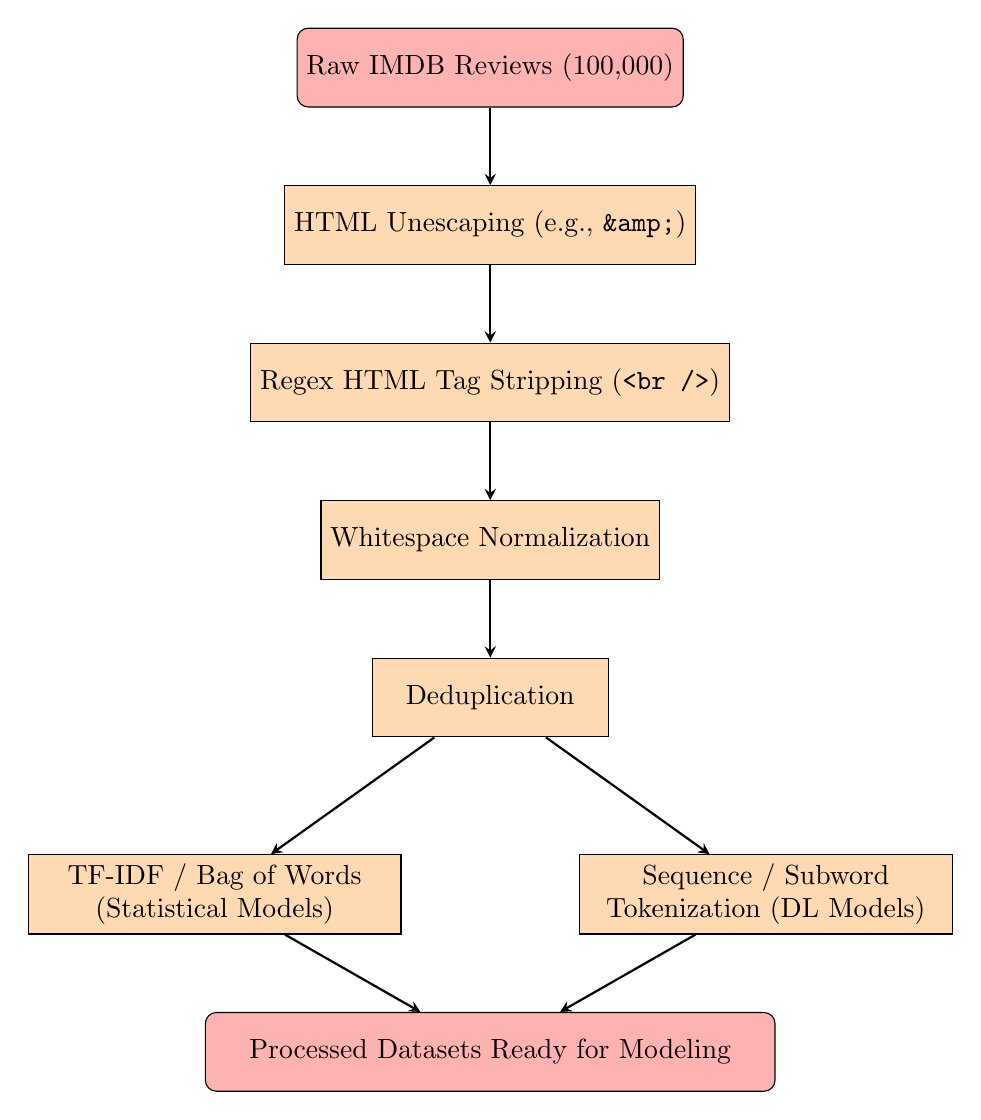
\begin{tikzpicture}[node distance=2cm]

\node (raw) [startstop] {Raw IMDB Reviews (100,000)};
\node (pro1) [process, below of=raw] {HTML Unescaping (e.g., \texttt{\&amp;})};
\node (pro2) [process, below of=pro1] {Regex HTML Tag Stripping (\texttt{<br />})};
\node (pro3) [process, below of=pro2] {Whitespace Normalization};
\node (pro4) [process, below of=pro3] {Deduplication};
\node (pathA) [process, below of=pro4, xshift=-3.5cm, yshift=-0.5cm, text width=4.5cm] {TF-IDF / Bag of Words (Statistical Models)};
\node (pathB) [process, below of=pro4, xshift=3.5cm, yshift=-0.5cm, text width=4.5cm] {Sequence / Subword Tokenization (DL Models)};
\node (out) [startstop, below of=pro4, yshift=-2.5cm, text width=7cm] {Processed Datasets Ready for Modeling};

\draw [arrow] (raw) -- (pro1);
\draw [arrow] (pro1) -- (pro2);
\draw [arrow] (pro2) -- (pro3);
\draw [arrow] (pro3) -- (pro4);
\draw [arrow] (pro4) -- (pathA);
\draw [arrow] (pro4) -- (pathB);
\draw [arrow] (pathA) -- (out);
\draw [arrow] (pathB) -- (out);

\end{tikzpicture}
\caption{Data Preprocessing and Feature Extraction Pipeline}
\label{fig:pipeline}
\end{figure}

The comprehensive pipeline highlighted in Figure \ref{fig:pipeline} demonstrates the end-to-end progression from raw textual data to numerical representations. To ensure high-quality model training, the following steps were systematically applied:

\begin{itemize}
    \item \textbf{HTML Unescaping:} The raw dataset contained encoded HTML entities (e.g., \texttt{\&amp;}, \texttt{\&quot;}). These were decoded back into standard ASCII characters to restore the original linguistic intent of the reviewers.
    \item \textbf{Regex HTML Tag Stripping:} As the data was scraped from a web platform, aggressive HTML tags (most notably \texttt{<br />}) were embedded throughout the text. Regular expressions were utilized to strip these structural tags without deleting the surrounding words.
    \item \textbf{Whitespace Normalization:} After tag removal, the text suffered from inconsistent spacing and hidden newline characters. All whitespace was normalized to single spaces, ensuring that identical words were not treated differently due to invisible spacing artifacts.
    \item \textbf{Deduplication:} A critical audit revealed duplicate reviews (96 in the training set, 199 in the testing set). Strict deduplication was enforced to prevent the models from artificially memorizing repeated samples and to eliminate the risk of data leakage.
    \item \textbf{Architecture-Specific Vectorization:} Because models cannot process raw strings, the cleaned text was numerically transformed. Crucially, this step diverged based on the target architecture:
    \begin{itemize}
        \item \textit{Statistical Models (Naive Bayes, XGBoost, LR, K-Means):} Transformed using Bag of Words and TF-IDF to capture frequency while penalizing generic stopwords.
        \item \textit{Deep Learning Models (LSTM, BERT):} Transformed using integer sequence encoding (LSTM) and subword WordPiece tokenization (BERT) to preserve sequential structure and dense contextual relationships.
    \end{itemize}
\end{itemize}

\section*{Exploratory Data Analysis}
A comprehensive EDA across all dataset variants revealed:

\subsection*{N-Gram Analysis}
Unigrams provided minimal discriminative power, as generic stopwords dominated the vocabulary. In contrast, bigram analysis surfaced highly discriminative phrases (e.g., ``worst movie'' vs. ``highly recommend''), heavily influencing the TF-IDF vectorization strategy used in the Logistic Regression and XGBoost models.

\subsection*{Punctuation and Sentiment Intensity}
Regression analysis uncovered a strong correlation between punctuation usage and sentiment extremity. 1-star reviews contained significantly more exclamation marks and ALL-CAPS text than 10-star reviews, indicating negative sentiment is expressed more ``aggressively.''

\subsection*{Review Length Distribution}
Analysis revealed a U-shaped distribution: reviews with extreme ratings (1-star and 10-star) were substantially longer than moderate reviews, indicating polarized opinions motivate more detailed writing.

\section*{Conclusion}
The preprocessing and EDA phases established a clean, well-characterized foundation for all downstream modeling tasks. The insights gathered, particularly regarding n-grams and meta-features, were critical for designing the subsequent regression and clustering models.

\end{document}
